% Options for packages loaded elsewhere
\PassOptionsToPackage{unicode}{hyperref}
\PassOptionsToPackage{hyphens}{url}
\documentclass[
  brazilian,
  11pt,
]{article}
\usepackage{xcolor}
\usepackage[margin=2.5cm]{geometry}
\usepackage{amsmath,amssymb}
\setcounter{secnumdepth}{5}
\usepackage{iftex}
\ifPDFTeX
  \usepackage[T1]{fontenc}
  \usepackage[utf8]{inputenc}
  \usepackage{textcomp} % provide euro and other symbols
\else % if luatex or xetex
  \usepackage{unicode-math} % this also loads fontspec
  \defaultfontfeatures{Scale=MatchLowercase}
  \defaultfontfeatures[\rmfamily]{Ligatures=TeX,Scale=1}
\fi
\usepackage{lmodern}
\ifPDFTeX\else
  % xetex/luatex font selection
\fi
% Use upquote if available, for straight quotes in verbatim environments
\IfFileExists{upquote.sty}{\usepackage{upquote}}{}
\IfFileExists{microtype.sty}{% use microtype if available
  \usepackage[]{microtype}
  \UseMicrotypeSet[protrusion]{basicmath} % disable protrusion for tt fonts
}{}
\makeatletter
\@ifundefined{KOMAClassName}{% if non-KOMA class
  \IfFileExists{parskip.sty}{%
    \usepackage{parskip}
  }{% else
    \setlength{\parindent}{0pt}
    \setlength{\parskip}{6pt plus 2pt minus 1pt}}
}{% if KOMA class
  \KOMAoptions{parskip=half}}
\makeatother
\usepackage{longtable,booktabs,array}
\usepackage{calc} % for calculating minipage widths
% Correct order of tables after \paragraph or \subparagraph
\usepackage{etoolbox}
\makeatletter
\patchcmd\longtable{\par}{\if@noskipsec\mbox{}\fi\par}{}{}
\makeatother
% Allow footnotes in longtable head/foot
\IfFileExists{footnotehyper.sty}{\usepackage{footnotehyper}}{\usepackage{footnote}}
\makesavenoteenv{longtable}
\usepackage{graphicx}
\makeatletter
\newsavebox\pandoc@box
\newcommand*\pandocbounded[1]{% scales image to fit in text height/width
  \sbox\pandoc@box{#1}%
  \Gscale@div\@tempa{\textheight}{\dimexpr\ht\pandoc@box+\dp\pandoc@box\relax}%
  \Gscale@div\@tempb{\linewidth}{\wd\pandoc@box}%
  \ifdim\@tempb\p@<\@tempa\p@\let\@tempa\@tempb\fi% select the smaller of both
  \ifdim\@tempa\p@<\p@\scalebox{\@tempa}{\usebox\pandoc@box}%
  \else\usebox{\pandoc@box}%
  \fi%
}
% Set default figure placement to htbp
\def\fps@figure{htbp}
\makeatother
\ifLuaTeX
\usepackage[bidi=basic]{babel}
\else
\usepackage[bidi=default]{babel}
\fi
% get rid of language-specific shorthands (see #6817):
\let\LanguageShortHands\languageshorthands
\def\languageshorthands#1{}
\setlength{\emergencystretch}{3em} % prevent overfull lines
\providecommand{\tightlist}{%
  \setlength{\itemsep}{0pt}\setlength{\parskip}{0pt}}
\usepackage{float}
\usepackage{booktabs}
\usepackage{longtable}
\usepackage{array}
\usepackage{caption}
\usepackage{setspace}
\usepackage{indentfirst}
\usepackage{titling}
\usepackage{graphicx}
\usepackage{xcolor}
\onehalfspacing
\usepackage{bookmark}
\IfFileExists{xurl.sty}{\usepackage{xurl}}{} % add URL line breaks if available
\urlstyle{same}
\hypersetup{
  pdflang={pt-BR},
  hidelinks,
  pdfcreator={LaTeX via pandoc}}

\author{}
\date{\vspace{-2.5em}22/06/2026}

\begin{document}

\begin{titlepage}
\centering

\vspace*{2.5cm}

{\Large Universidade de São Paulo \par}

\vspace{0.5cm}

{\large Faculdade de Economia, Administração, Contabilidade e Atuária \par}

\vspace{2.2cm}

{\Huge \textbf{Avaliação da Informatização no Desempenho Escolar} \par}

\vspace{2.5cm}

{\large Felipe Ferreira Alexandre 13693144  \par}

\vspace{0.4cm}

{\large Andrei  \par}

\vspace{0.4cm}

{\large 22/06/2026  \par}

\vfill

\end{titlepage}

\subsection{1. Construção da base
descritiva}\label{construuxe7uxe3o-da-base-descritiva}

\subsection{2. Tabela curta de cobertura da
amostra}\label{tabela-curta-de-cobertura-da-amostra}

Essa tabela é útil no trabalho porque mostra se temos número suficiente
de escolas por ano e etapa.

\begin{longtable}[]{@{}
  >{\raggedleft\arraybackslash}p{(\linewidth - 12\tabcolsep) * \real{0.0704}}
  >{\raggedright\arraybackslash}p{(\linewidth - 12\tabcolsep) * \real{0.2113}}
  >{\raggedleft\arraybackslash}p{(\linewidth - 12\tabcolsep) * \real{0.1127}}
  >{\raggedleft\arraybackslash}p{(\linewidth - 12\tabcolsep) * \real{0.0704}}
  >{\raggedleft\arraybackslash}p{(\linewidth - 12\tabcolsep) * \real{0.1268}}
  >{\raggedleft\arraybackslash}p{(\linewidth - 12\tabcolsep) * \real{0.2113}}
  >{\raggedleft\arraybackslash}p{(\linewidth - 12\tabcolsep) * \real{0.1972}}@{}}
\caption{Cobertura da amostra por ano e etapa escolar}\tabularnewline
\toprule\noalign{}
\begin{minipage}[b]{\linewidth}\raggedleft
ano
\end{minipage} & \begin{minipage}[b]{\linewidth}\raggedright
anos\_escolares
\end{minipage} & \begin{minipage}[b]{\linewidth}\raggedleft
escolas
\end{minipage} & \begin{minipage}[b]{\linewidth}\raggedleft
obs
\end{minipage} & \begin{minipage}[b]{\linewidth}\raggedleft
com\_ideb
\end{minipage} & \begin{minipage}[b]{\linewidth}\raggedleft
com\_matematica
\end{minipage} & \begin{minipage}[b]{\linewidth}\raggedleft
com\_portugues
\end{minipage} \\
\midrule\noalign{}
\endfirsthead
\toprule\noalign{}
\begin{minipage}[b]{\linewidth}\raggedleft
ano
\end{minipage} & \begin{minipage}[b]{\linewidth}\raggedright
anos\_escolares
\end{minipage} & \begin{minipage}[b]{\linewidth}\raggedleft
escolas
\end{minipage} & \begin{minipage}[b]{\linewidth}\raggedleft
obs
\end{minipage} & \begin{minipage}[b]{\linewidth}\raggedleft
com\_ideb
\end{minipage} & \begin{minipage}[b]{\linewidth}\raggedleft
com\_matematica
\end{minipage} & \begin{minipage}[b]{\linewidth}\raggedleft
com\_portugues
\end{minipage} \\
\midrule\noalign{}
\endhead
\bottomrule\noalign{}
\endlastfoot
2015 & anos\_finais & 3991 & 3991 & 3536 & 3536 & 3536 \\
2017 & anos\_finais & 3991 & 3991 & 2267 & 2267 & 2267 \\
2019 & anos\_finais & 3991 & 3991 & 3246 & 3246 & 3246 \\
2021 & anos\_finais & 4000 & 4000 & 2927 & 2927 & 2927 \\
2023 & anos\_finais & 4013 & 4013 & 3425 & 3426 & 3426 \\
2015 & anos\_iniciais & 1977 & 1977 & 1452 & 1452 & 1452 \\
2017 & anos\_iniciais & 1977 & 1977 & 1367 & 1367 & 1367 \\
2019 & anos\_iniciais & 1977 & 1977 & 1420 & 1420 & 1420 \\
2021 & anos\_iniciais & 1979 & 1979 & 1285 & 1285 & 1285 \\
2023 & anos\_iniciais & 1984 & 1984 & 1310 & 1310 & 1310 \\
2017 & todos (1-4) & 3709 & 3709 & 1491 & 1491 & 1491 \\
2019 & todos (1-4) & 3709 & 3709 & 2565 & 2565 & 2565 \\
2021 & todos (1-4) & 3728 & 3728 & 1354 & 1354 & 1354 \\
2023 & todos (1-4) & 3746 & 3746 & 2862 & 2863 & 2863 \\
\end{longtable}

\subsection{3. Composição dos
tratamentos}\label{composiuxe7uxe3o-dos-tratamentos}

\subsubsection{3.1 CMSP}\label{cmsp}

\begin{longtable}[]{@{}lrrr@{}}
\caption{Composição das escolas segundo exposição ao
CMSP}\tabularnewline
\toprule\noalign{}
grupo\_cmsp & escolas & intensidade\_media & intensidade\_mediana \\
\midrule\noalign{}
\endfirsthead
\toprule\noalign{}
grupo\_cmsp & escolas & intensidade\_media & intensidade\_mediana \\
\midrule\noalign{}
\endhead
\bottomrule\noalign{}
\endlastfoot
Tratada CMSP & 5480 & 110504627 & 78559772 \\
Nunca tratada CMSP & 479 & 0 & 0 \\
\end{longtable}

\subsubsection{3.2 Informatização}\label{informatizauxe7uxe3o}

\begin{longtable}[]{@{}lrr@{}}
\caption{Composição das escolas segundo trajetória de
informatização}\tabularnewline
\toprule\noalign{}
grupo\_info & escolas & pct \\
\midrule\noalign{}
\endfirsthead
\toprule\noalign{}
grupo\_info & escolas & pct \\
\midrule\noalign{}
\endhead
\bottomrule\noalign{}
\endlastfoot
Tornou-se informatizada & 4251 & 82.78 \\
Reverte tratamento & 616 & 12.00 \\
Nunca informatizada & 239 & 4.65 \\
NA & 28 & 0.55 \\
Já informatizada no início & 1 & 0.02 \\
\end{longtable}

\subsection{4. Tendências prévias:
CMSP}\label{tenduxeancias-pruxe9vias-cmsp}

Essa é uma das figuras mais importantes do trabalho. Ela compara a
trajetória média dos resultados \textbf{antes da exposição ao CMSP}.

\begin{center}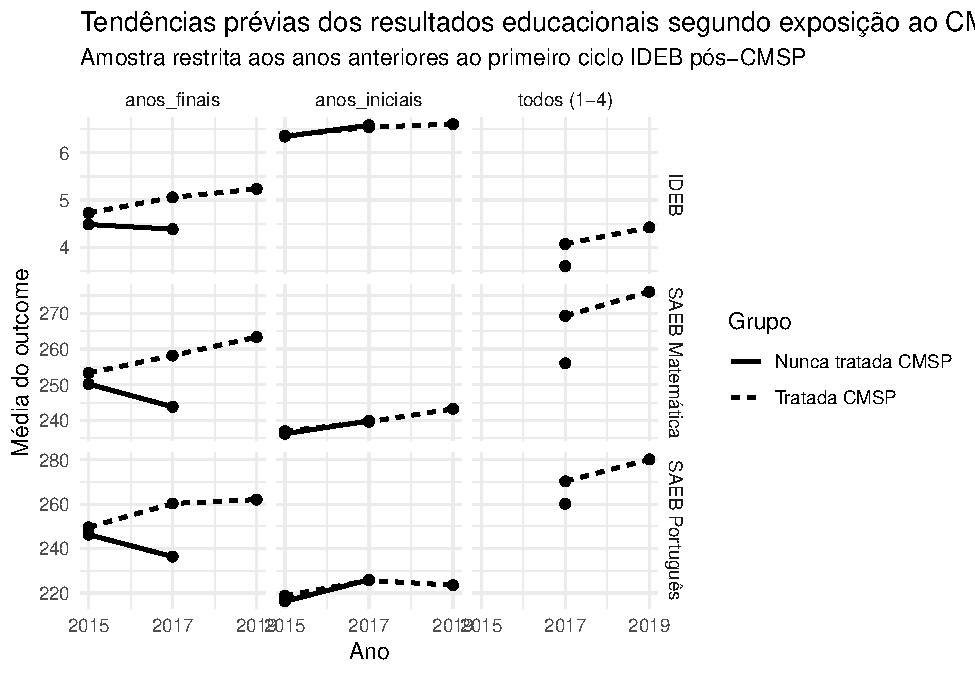
\includegraphics[width=0.85\linewidth]{avaliacao_impacto_base_painel_files/figure-latex/tendencias_previas_cmsp-1} \end{center}

\end{document}
